
\newcommand{\figureQuadpolBandsExample}[2]
{
\begin{figure}[#1] 
\centering
\subcaptionbox{Polarisation HH\label{fig:Polarisation-HH}}
{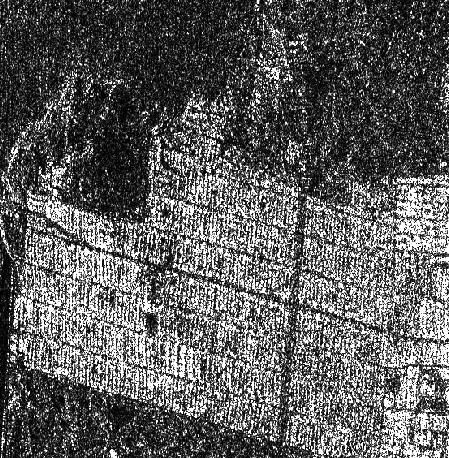
\includegraphics[width=#2 \linewidth]{figures/Chap2/polsar_bands_sf/RS2-SLC-FQ9-ASC-09-Apr-2008_02_Intensity_HH-diagram.jpg}}
\subcaptionbox{Polarisation HV\label{fig:Polarisation-HV}}
{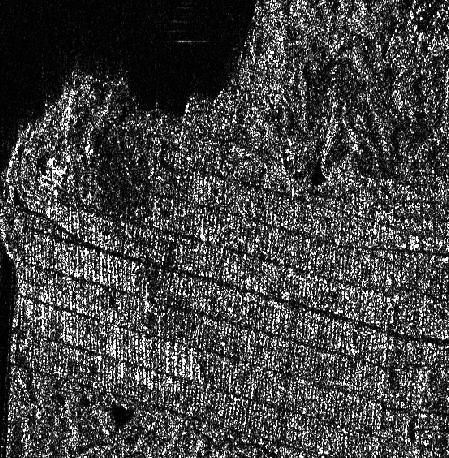
\includegraphics[width=#2  \linewidth]{figures/Chap2/polsar_bands_sf/RS2-SLC-FQ9-ASC-09-Apr-2008_02_Intensity_HV-diagram.jpg}}
\subcaptionbox{Polarisation VH\label{fig:Polarisation-VH}}
{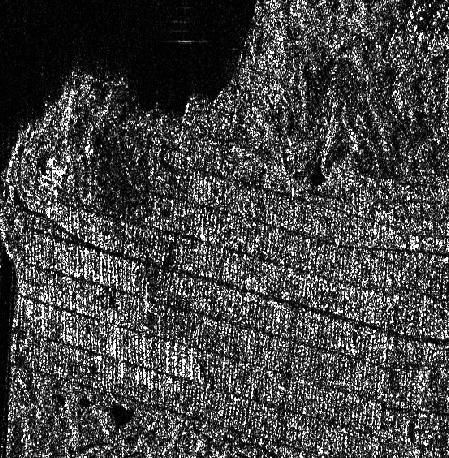
\includegraphics[width=#2  \linewidth]{figures/Chap2/polsar_bands_sf/RS2-SLC-FQ9-ASC-09-Apr-2008_02_Intensity_VH-diagram.jpg}}
\subcaptionbox{Polarisation VV\label{fig:Polarisation-VV}}
{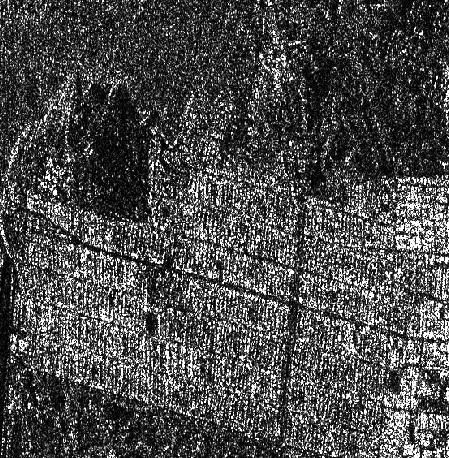
\includegraphics[width=#2  \linewidth]{figures/Chap2/polsar_bands_sf/RS2-SLC-FQ9-ASC-09-Apr-2008_02_Intensity_VV-diagram.jpg}}
 \caption
        {\small Les quatre bandes polarimétriques d'une image QuadPol RADARSAT-2 (San Francisco)} 
        \label{fig:polsar-bands-diagram}
\end{figure}
}